\section{分析框架}
\label{sec:factory}

\noindent
为了以统一、公平的方式系统分析不同调度策略，我们实现了一个灵活的 LLM 调度分析框架——{\sys}。
推动 {\sys} 设计的原因有两点：
(1) 现有策略分散在不同服务系统的具体实现中（既包括开源实现，也包括闭源实现），因此很难进行真正可比的横向分析。
例如，AIBrix~\cite{aibrix} 中 vLLM 策略的 Go 实现，由于后来被确认的性能缺陷~\cite{vllm-bug}，比 vLLM 的 Python 实现~\cite{vllm-code} 快 6.2\,$\times$。
与此同时，我们基于 Rust 的实现，在使用相同 vLLM 策略的情况下，又比 AIBrix 快 1.2\,$\times$。
(2) 统一框架还能简化新策略的实现与比较：尽管细节复杂，现有所有策略本质上都可以归结为依据实例指标计算调度分数。
通过提供统一的指标工厂，我们的框架只需几行代码就可以探索新的策略（下文将介绍）。

\begin{figure}[!t]
%        \hspace{-2mm}
        \begin{minipage}{1\linewidth}
        \centering
        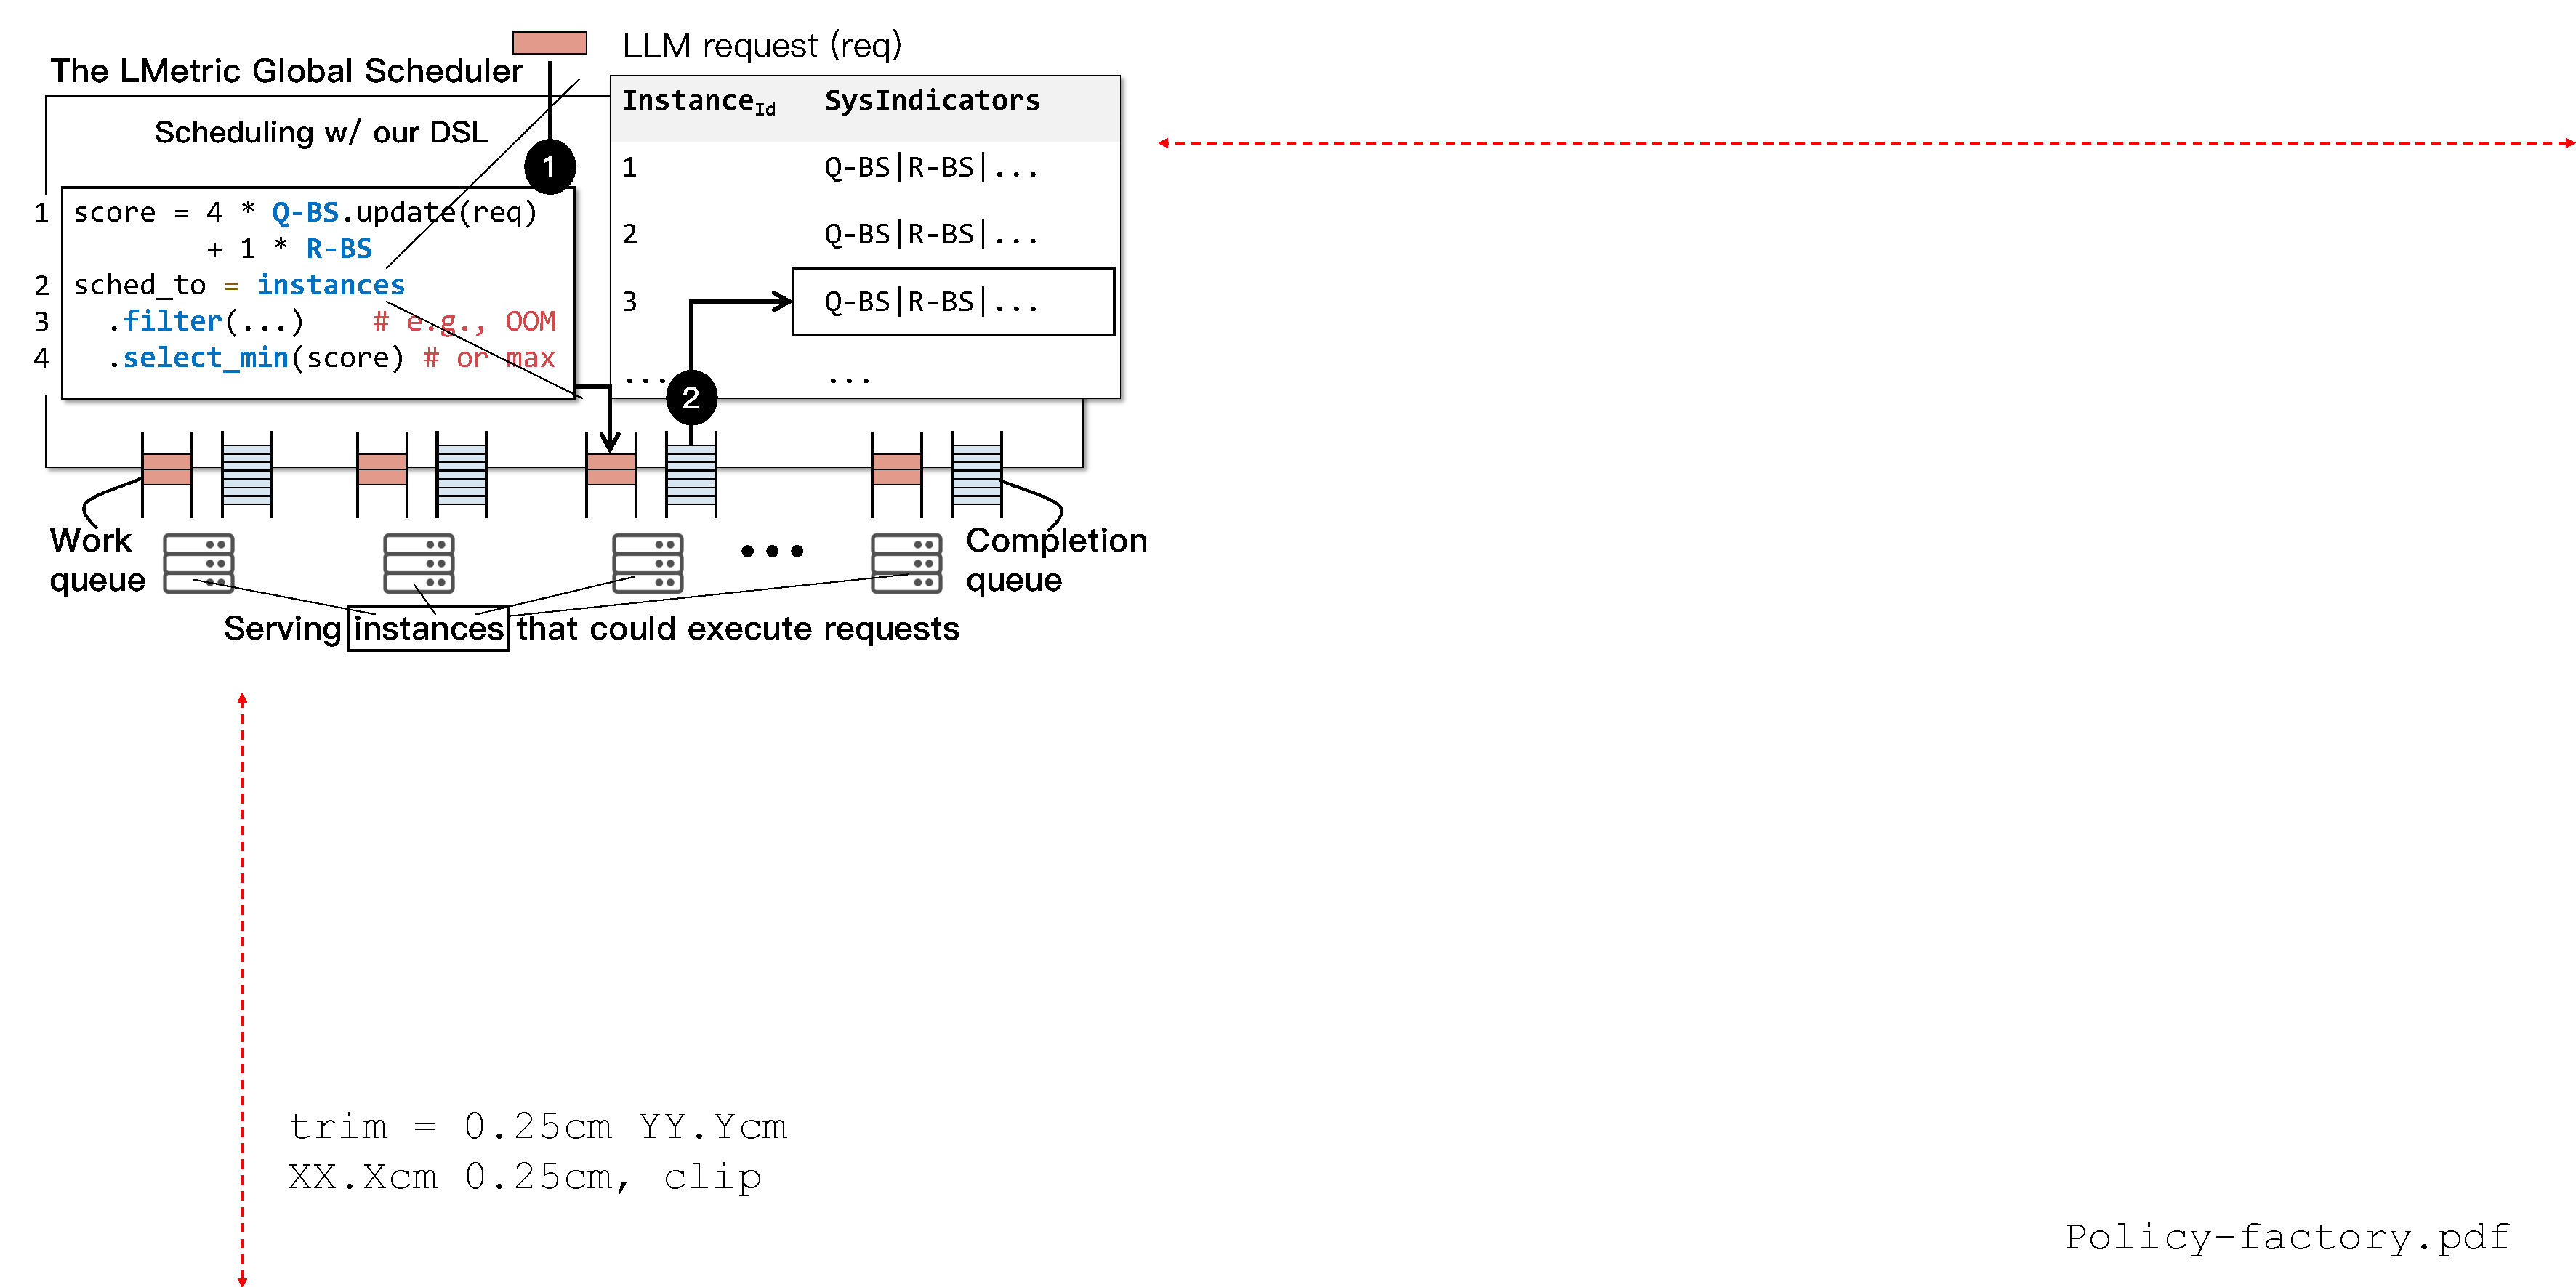
\includegraphics[width=0.95\linewidth, trim=0.25cm 14.75cm 33cm 0.25cm, clip]{figs/policy-factory.pdf}
        \end{minipage} \\[5pt]
        \begin{minipage}{1\linewidth}
        \caption{\small{%
        {\sys} 指标工厂的系统架构，以及其面向调度算法的编程模型。
        }}
        \label{fig:factory}
        \end{minipage} \\[-10pt]
        \end{figure}

\stitle{指标工厂。\,}
{\sys} 是一个使用 Rust 实现的独立推理路由器，可以与任意 LLM 服务引擎协同工作。
如 {\fig{fig:factory}} 所示，其核心组件是一个\emph{指标工厂}：它能够自动收集并在需要时计算不同调度策略所需的指标。
选择 Rust 使得 {\sys} 具备极高的效率与鲁棒性。
为了获得高可扩展性，指标收集被搭载在实例返回响应这一过程中。
例如，{\sys} 会与每个 vLLM 实例维持长连接；当 vLLM 返回响应时，{\sys} 会从响应头中提取所需指标，并更新指标工厂中对应的条目。

\stitle{编程模型。\,}
{\sys} 提供了一个简单的 API 来实现不同调度策略。
具体而言，所有策略本质上都是先为每个实例计算一个分数，再将请求路由到分数最优（例如最小或最大）的实例。
我们的 API 允许开发者基于指标工厂支持的“每实例符号指标”，用少量表达式定义分数函数。
{\fig{fig:factory}} 中第 1 行给出了 vLLM~\cite{vllm-code} 所采用的一个具体策略：
它将 \texttt{Q-BS}（queued batch size，即实例队列中排队请求的数量）与 \texttt{R-BS}（实例上正在运行的请求数量）做加权求和，作为调度分数。
在定义好分数函数之后，当系统需要决定新请求应被路由到哪里时（第 4 行），
{\sys} 会先并行地从指标工厂中读取并计算各实例的具体指标值，再推导出所有实例的分数，最后把请求路由到分数最小的实例。
